\documentclass[11pt,twocolumn]{article}
\usepackage{amsmath}
\usepackage{graphicx}
\usepackage{color}
\usepackage{epsfig}
\usepackage{float}
\usepackage{algorithm}
\usepackage[noend]{algorithmic} 
\usepackage{float} 
\setlength\topmargin{-0.5in}
\setlength\headsep{0in}
\setlength\textheight{9.5in}
\definecolor{gray}{rgb}{0.9,0.9,0.9}
\newcommand{\todo}[1]{\textcolor{red}{\textbf{#1}}}
\newcommand{\tbf}{\textbf}
\newcommand{\tit}{\textit}
\newcommand{\ds}{\displaystyle}
\newcommand{\argmax}{\operatornamewithlimits{argmax}}

%GOOD FOR POSITIONING THE IMAGES AND THE TABLES WELL??????????
\renewcommand\floatpagefraction{.9}
\renewcommand\topfraction{.9}
\renewcommand\bottomfraction{.9}
\renewcommand\textfraction{.1}   
\setcounter{totalnumber}{50}
\setcounter{topnumber}{50}
\setcounter{bottomnumber}{50}
%?????????????????????????????????????????????????????????????

\title{\tbf{Dirty Money:}\\\tbf{Feature selection using AdaBoost}}
\author{J. van Turnhout (0312649) jturnhou@science.uva.nl, 
	 \\ N. Raiman (0336696) nraiman@science.uva.nl, 
	 \\ S. L. Pintea (6109969) s.l.pintea@student.uva.nl}

\begin{document}
\begin{titlepage}
	\maketitle
	\vspace*{300px}
	\centering
	\huge{\textbf{CONFIDENTIAL}}
 \end{titlepage}

	
	\begin{abstract}
		In the month January of 2010 a project on the classification of
		the fitness of money was proposed. During this month we have tested and
		implemented various techniques to handle the problem of money classification.
		The results from our experiment show promising development comparing to the
		current state of research.
		
		In the below sections we have described the approaches that we
		have tried and the results obtained for each one of them.
	\end{abstract}
	
	\section{Introduction}
		The goal of this project is to research several techniques that have a potential to distinguish between clean bills and dirty bills. In order to achieve this goal we had to think of what are the representative features of dirt that can be found on money bills and what techniques can be applied to model this.
		 		
		The main techniques used in this project are: \emph{PCA}, \emph{Haar-like features}, \emph{Convolution with predefined kernels}, \emph{edge-detection} and \emph{intensity} distributions. All of these techniques have been analyzed on the image data using a machine learning technique called Adaptive Boosting, also referred to in literature as AdaBoost \cite{Ada}.
		
		In section \ref{sec:Background}, related work on the project is discussed. In section \ref{sec:Methods}, the implementation of the \emph{AdaBoost} algorithm applied on the different techniques \emph{Haar-like features}, \emph{convolution with kernels}, \emph{PCA}, \emph{SVM}, \emph{AdaBoost}, \emph{edge detection} and \emph{intensity} are discussed. We explain our experiments and their results in section \ref{sec:results}. Finally, we conclude in section \ref{sec:conclusion} and propose some topics for future research.

	\section{Background}\label{sec:Background}
		In Europe a lot of different factories produce Euro bills using different ink and paper. This makes the task of detecting dirty bills hard because looking at the global features will not work perfectly due to these small differences in printing. In The Netherlands, on average bills return 2 to 3 times a year to the Dutch National Bank (DNB), in total of 1.1 billion bills a year. 

		The current approach used in the DNB is to measure the reflection of the bill on a small area near the water mark. With this approach 30\% of all bills are destroyed in order to destroy 95\% of the dirty bills. In a first attempt to make this selection process more sophisticated global features (eigen-money) of clean and dirty bills are extracted using PCA analysis \cite{MoNuSt}. This approach improved on the results of the current method used by the DNB. For 5 Euro bills the error on clean bills was 12\%, on dirty bills 10.5\% and for 10 Euro the error on clean bills was 15\%, on dirty bills 7.5\%.  The implementation was again improved by learning more local features of the water mark region (also referred to as white patch) of the bill \cite{Geusebroek}.  For 5 Euro bills the error on clean bills was 3\%, on dirty bills 0\% and for 10 Euro the error on clean bills was 16\%, on dirty bills 6\%.
	\section{Methods}\label{sec:Methods}
		\subsection{Adaboost}\label{sec:Adaboost}
			The \emph{AdaBoost} algorithm will be used in combination with different techniques throughout this project, such as: \emph{PCA}, \emph{Haar-like features} and \emph{edge} and \emph{intensity} distributions over different regions.

AdaBoost is a machine learning technique which can be used in conjunction with various other learning algorithms. The idea is to have a (convex) set of weak classifiers (classifiers that perform at least better than random) and then minimize the total error over the training-set by finding the best classifier at each stage of the algorithm.

The theoretical basis of this algorithm is that given a set of models (or features), \emph{M}, the algorithm will determine the subset of \emph{T} models that	 are the best for distinguishing between the two classes (clean and dirty bills). Thus, \emph{AdaBoost} will learn the most representative features of the two classes. The algorithm for determining the best models is shown in \emph{Algorithm~\ref{AdaBoost}}. Another very important characteristic of this algorithm is the fact that it also specifies a method in which the models that were chosen as being the best, can be combined in order to give a strong classifier. The corresponding algorithm can be seen in \emph{Algorithm~\ref{AdaBoost_pred}}.

Note that although this algorithm looks slightly different, is equivalent to the one described in \cite{Haar}.
			
		\begin{algorithm}[!hbtp]
				\caption{AdaBoost learning features}
				\label{AdaBoost}
				\begin{algorithmic}[1]
				\medskip
				\STATE \tbf{function} AdaBoostLearn($T$, $M$, $S$) 
				\STATE {$T$ = nr. of hypothesis}
				\STATE {$M$ = Models}
				\STATE {$S$ = training-set, \{$(x_1,y_1),...(x_n,y_n)$\} \\ with $x_i \epsilon X$ and $y_i \epsilon \{-1, 1\}$ }
				\STATE {$D_{1(i)} \leftarrow \frac{1}{n}$, with $i=1,...,n$}
				\FOR {$t=1$ to $T$}
					\STATE {$error_t \leftarrow 0$}
					\FOR {$m \epsilon M$}
						\STATE {$h_j(x_i) \leftarrow predict(x_i)$ \%\tit{SVM or Gaussian distribution}}
						\STATE {$error_j \leftarrow \sum^n_{i=1}D_t(i)[y_i \neq h_j(x_i)]$}
						\IF {$error_j < error_t$}
							\STATE {$error_t \leftarrow error_j$}
							\STATE {$h_t \leftarrow h_j$}
						\ENDIF
					\ENDFOR
					\STATE {$\alpha_t \leftarrow 0.5 \cdot \log{\frac{1-error_t}{error_t}}$}
					\FOR {$i=1$ to $n$}
						\STATE {$D_{t+1}(i) \leftarrow \frac{D_t(i)\exp{-\alpha_t \cdot y_i \cdot h_t(x_i)}}{Z_t}$}
					\ENDFOR
				\ENDFOR
				\STATE {\tbf{return} $\alpha, h$}
				\end{algorithmic}
				\label{alg:AdaBoostLearn}
			\end{algorithm}

			\begin{algorithm}[!hbtp]
				\caption{AdaBoost Prediction}
				\label{AdaBoost_pred}
				\begin{algorithmic}[1]
				\medskip
				\STATE \tbf{function} AdaBoostPredict($\alpha$, $h$, $I$)
				\STATE { $\alpha$ = weights }
				\STATE { $h$ = weak classifiers}
				\STATE {$I$ = image}
				\STATE {$p$ = prediction} 
				\FOR {$t=1$ to $length(\alpha)$}
					\STATE $p \leftarrow p + \alpha_th_t(I)$
				\ENDFOR
				\STATE {\tbf{return} $sign(p)$}
				\end{algorithmic}
				\label{alg:AdaBoostPredict}
			\end{algorithm}

		\subsection{Haar-like features and convolution with Haar-like kernels}\label{sec:Haar}
			The \emph{Viola \& Jones} approach for object detection has been successfully applied to face recognition tasks. In previous projects, the use of PCA for classification is motivated by its application in face recognition. The use of Haar-like features has proven its purpose in this field as well and therefore it is plausible that the technique could be adapted to our problem. The final cascade used in the paper however was not implemented because the main idea of this cascade was not suitable for the purpose of this project. We have used the strong classifier computed in \emph{AdaBoost} as the final output.

			\begin{figure}[!hbtp]
				\fbox{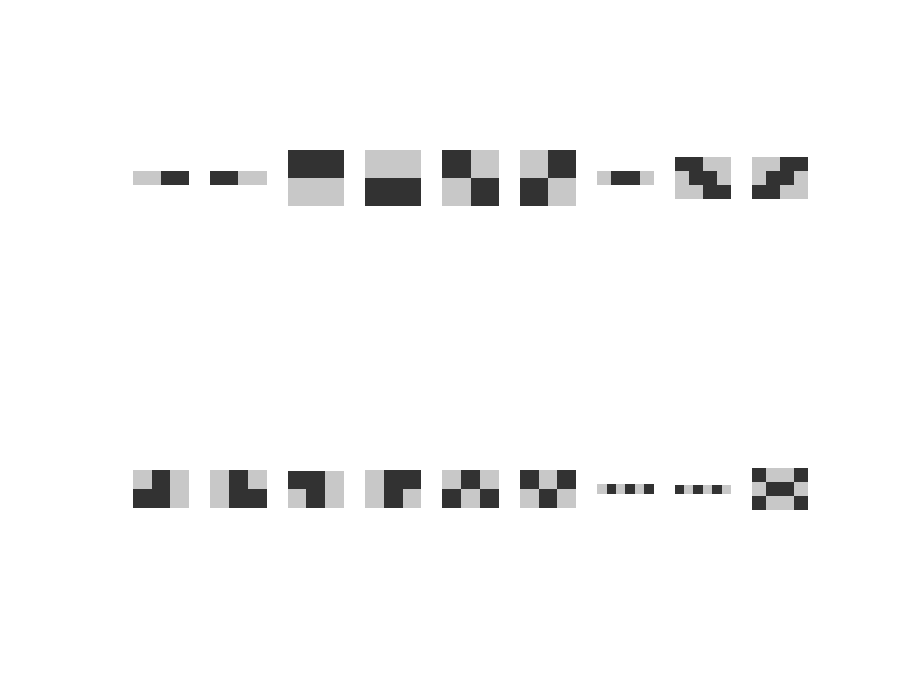
\epsfig{file=img/patterns.eps, width=0.9\linewidth}}
				\caption{Patterns}
				\label{patterns}
			\end{figure}

			The first step of the algorithm is defining the patterns, that are mainly matrices of different dimensions containing low and high values for intensity (-1 and 1). Figure \ref{patterns} indicates a subset of the patterns used. The algorithm used in the \emph{Viola \& Jones} article was designed to loop over all predefined patterns on each position in the image and convolve the specific region of the image with the patterns using the formula depicted in Figure \ref{patterns_formula}.
			
			\begin{figure}
				\fontfamily{ccr}\selectfont\small
				\caption{}
				\begin{tabular}{|lr|} \hline
					& \\[5pt]
					\textcolor{blue}{$\sum_x\sum_y Image(y:y+h,x:x+w) .* Pattern$} &\\[10pt]
					where: \emph{h} -- the heigh of the pattern &\\
					\hspace*{28px} \emph{w} -- the width of the pattern &\\[5pt] 
					\hline 
				\end{tabular}
				\label{patterns_formula}
			\end{figure}
			
			We have started by defining a large number of patterns of different sizes ($\approx$100 patterns), and filtered out those that gave bad results when used in the \emph{AdaBoost algorithm} for training the weak classifiers. The resulted values for each pattern and location in the image would then be used in \emph{AdaBoost} to train an \emph{SVM} classifier. 
			
			Taking into account the fact that the set of features generated by the algorithm for each pattern and each image was extremely large, the training took too much time. In order to solve this problem, we have decided to use random locations at which to convolve the patterns with a region of the image that would have the same size as the pattern. Figure~ \ref{Haar_features} indicates what \emph{AdaBoost} would choose as being the most representative 7 features for the front side and rear side of the bills.

			\begin{figure}[!hbtp]
				\centering
				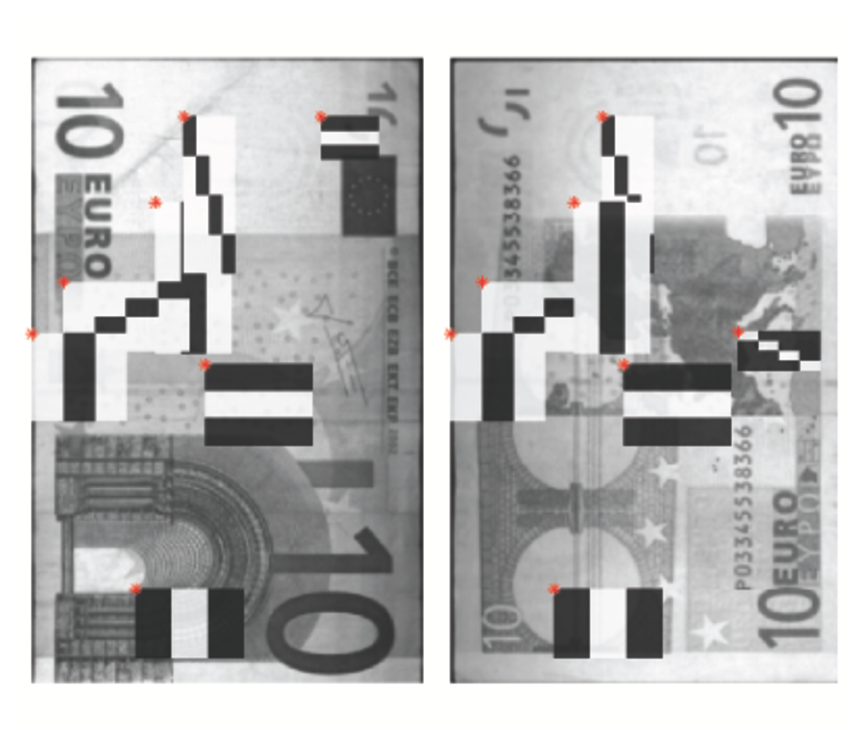
\epsfig{file=img/haar.eps, width=1\linewidth}
				\caption{Haar Features for Front and Rear}
				\label{Haar_features}
			\end{figure}

			The results obtained using \emph{Haar features} were not as	good as we would have expected them to be. An explanation for this may be the fact that the patterns defined were describing local features on pixel-level making it impossible to generalize to a more global level.
			
			The second approach that we have tried was to define a set of patterns as before, and to segment each image into smaller regions that would be, then, convolved with the patterns.
			
			We have tried using both non-overlapping segmentation of the images and 50\% overlapping one. Due to the fact that many essential pixel values (like those that would indicate the presence of dirt) may happen to be positioned on the line that separates two neighboring regions, it is possible that some information might be lost. As expected, the second method of dividing the images into regions gave better results compared to the first one.

			The resulted values obtained by summing the convolved values of the pixels represented the input set of features for the \emph{AdaBoost algorithm}. Figure \ref{convolved} will help getting a better understanding of how the result of convolving an image with a \emph{haar-like} feature looks like. In this image is plotted the result obtained when convolving a bill with a simple pattern such as: \textbf{[1 -1;-1 1]}.

			\begin{figure}[!hbtp]
				\centering
				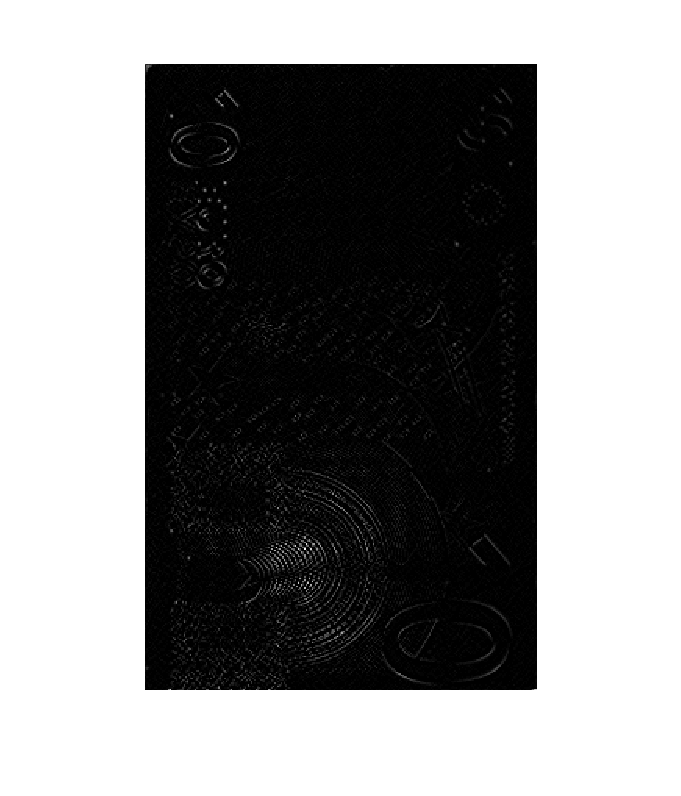
\epsfig{file=img/convolution.eps, width=0.5\linewidth}
				\caption{Convolution of an entire bill}
				\label{convolved}
			\end{figure}

			For establishing the set of the best \emph{T} features we have tried using both \emph{SVM} and \emph{Gaussian distributions}, and the results retrieved by the last one seemed slightly better than the ones obtained while using \emph{SVM}. In the case in which \emph{SVM} was used, a model was generated for each available feature. This model would give the best separation between the values corresponding to that feature for fit images and those for unfit images. In the case of the \emph{Gaussian distribution}, the \emph{mean} and \emph{covariance} of features corresponding to fit images were computed, respectively the mean and covariance for the features corresponding to unfit images. In order to determine the predicted class of the input images we have tried two methods.

			In the first method we would simply compute the \emph{mean} and \emph{covariance} for the values corresponding to fit, respectively unfit values for a specific feature. During testing, for each input value, we would compare the two numbers returned by \emph{Gaussian density function} for fit, respectively unfit and we would choose the predicted class to be the maximum of the two.

			The second method was applying \emph{Naive Bayes} in order to make use of the prior knowledge available. We know that in a real-life situation there are always more fit bills than unfit ones and we would like to use this information to improve our classifiers. The predicted class was defined by using the \emph{MAP} (maximum aposterior probability) estimation. The formula for computing the maximum aposterior probability for fit, respectively unfit class is depicted in Figure \ref{MAP_formula}.

			\begin{figure}[!hbtp] \fontfamily{ccr}\selectfont\small
				\caption{}
				\begin{tabular}{|lr|} \hline
					&\\[5pt]
					\textcolor{blue}{$argmax_{\theta_{fit}}P(\theta_{fit}\mid X) = $} &\\[5pt]
					\hspace*{50px}\textcolor{blue}{$\frac{P(\theta_{fit})*P(X\mid \theta_{fit})}{P(\theta_{fit})*P(X\mid \theta_{fit}) + P(\theta_{unfit})*P(X\mid \theta_{unfit})}$} &\\[15pt]
					\textcolor{blue}{$argmax_{\theta_{unfit}}P(\theta_{unfit}\mid X) = $} &\\[5pt]
					\hspace*{50px}\textcolor{blue}{$\frac{P(\theta_{unfit})*P(X\mid \theta_{unfit})}{P(\theta_{fit})*P(X\mid \theta_{fit}) + P(\theta_{unfit})*P(X\mid \theta_{unfit})}$} &\\[10pt]
			\hline
			\end{tabular}
					where: 
					\begin{itemize}
					\item $P(\theta_{fit}), P(\theta_{unfit})$ -- marginal probabilities of
						"fit" class, respectively "unfit" class
					\item $\theta_{fit}, \theta_{unfit}$ -- the parameters of the classes (mean
						and covariance)
					\item $P(X\mid \theta_{fit}),P(X\mid \theta_{unfit})$ -- the conditional
						probabilities of the two classes (representing normal distributions)
					\end{itemize} 
			\label{MAP_formula}
			\end{figure}

			It can be easily shown that the values of the parameters $\theta$ for a normal distribution (mean and covariance) that would maximize the probability of the classes are exactly the corresponding formulas indicated in Figure \ref{mu_sigma}.

			\emph{ \begin{figure}[!hbtp] \fontfamily{ccr}\selectfont\small
				\caption{}
				\begin{tabular}{|lr|} \hline
						&\\[5pt]	
						\textcolor{blue}{$\mu$ = $\sum_i \frac{x_i}{\mid X \mid}$}&\\
						\textcolor{blue}{$\sigma$ = $\frac{(X - \mu)(X - \mu)^T}{\mid X \mid}$} &\\[10pt]  
						where X -- the training data set &\\
						\hspace*{28px} $\mu$ -- the mean &\\
						\hspace*{28px} $\sigma$ -- the covariance &\\[5pt]
				\hline
				\end{tabular}
				\label{mu_sigma}
			\end{figure}
			}
			The second technique used for determining the predicted class of the data given the parameters seemed to provides slightly better results in practice	due to the fact that it also incorporates some prior knowledge of the data.

			For this approach we have used two classifiers: one for the rear side and another for the front side of the bills and the predictions	given by the two classifiers were combined into a third one using Naive Bayes.

			In order to create the final model, we have tried two different methods:
			\begin{itemize}
				\item the first one was essentially just choosing the best model (the one
				that gives the minimum error) throughout all the repetitions and all the
				rounds in the validation;
				\item the second method was to use a system of voting -- each time a
				feature was chosen by the \emph{AdaBoost} algorithm, it would receive a
				vote. In the end the top \emph{T} most voted features throughout all the
				validation rounds and all the repetitions would be chosen from the
				best model found. The corresponding weights would be generate by taking the
				mean of the features\rq\@ $\alpha$-weights computed in the \emph{AdaBoost}
				algorithm;
			\end{itemize}

			As we would have expected, the voting method for defining the best model, proved to give better results in this case so it was chosen to be applied.

		\subsection{PCA and SVM}\label{sec:PCA}
			In previous research, the use of SVM in combination with PCA already gave great error reduction on both the 5 and 10 Euro bills. The best results were conducted from performing PCA on the white-patch area only, and propagate the projections through the SVM. PCA on the white-patch as well as the whole bill made it possible to reduce the data from a dimensionality equal to the number of pixels of the respective area to only a 30 components. This reduction ensures faster training and classification with SVM. The idea is to identify more regions with similar discriminative features as the white-patch. This is done by dividing the bill up in an arbitrary number of regions, and performing PCA for each of these regions in all the bills. The PCA segments then can be used to train SVM models for each segment. These SVM models in combination with their respective PCA segments in turn can be used as weak classifiers in AdaBoost. The dimensions for division are chosen using empirical evidence of the error rates, and as to be expected the segments cannot be too local for PCA to work.

		\subsection{Intensity and Edge distributions}\label{sec:Intensity_Edge}
			Next to the more complex approaches we decided to implement also two more simple techniques, based on the intensities on the image and on the edges on the bill. After plotting the average intensity and edge count for the hole bills we were convinced these simple approaches should work well. Figure \ref{histograms} shows on the left the average intensity plot and on the right the plot of the edge count for 5 Euro (on top) and for 10 Euro.

			\begin{figure}[!hbtp]
				\centering
				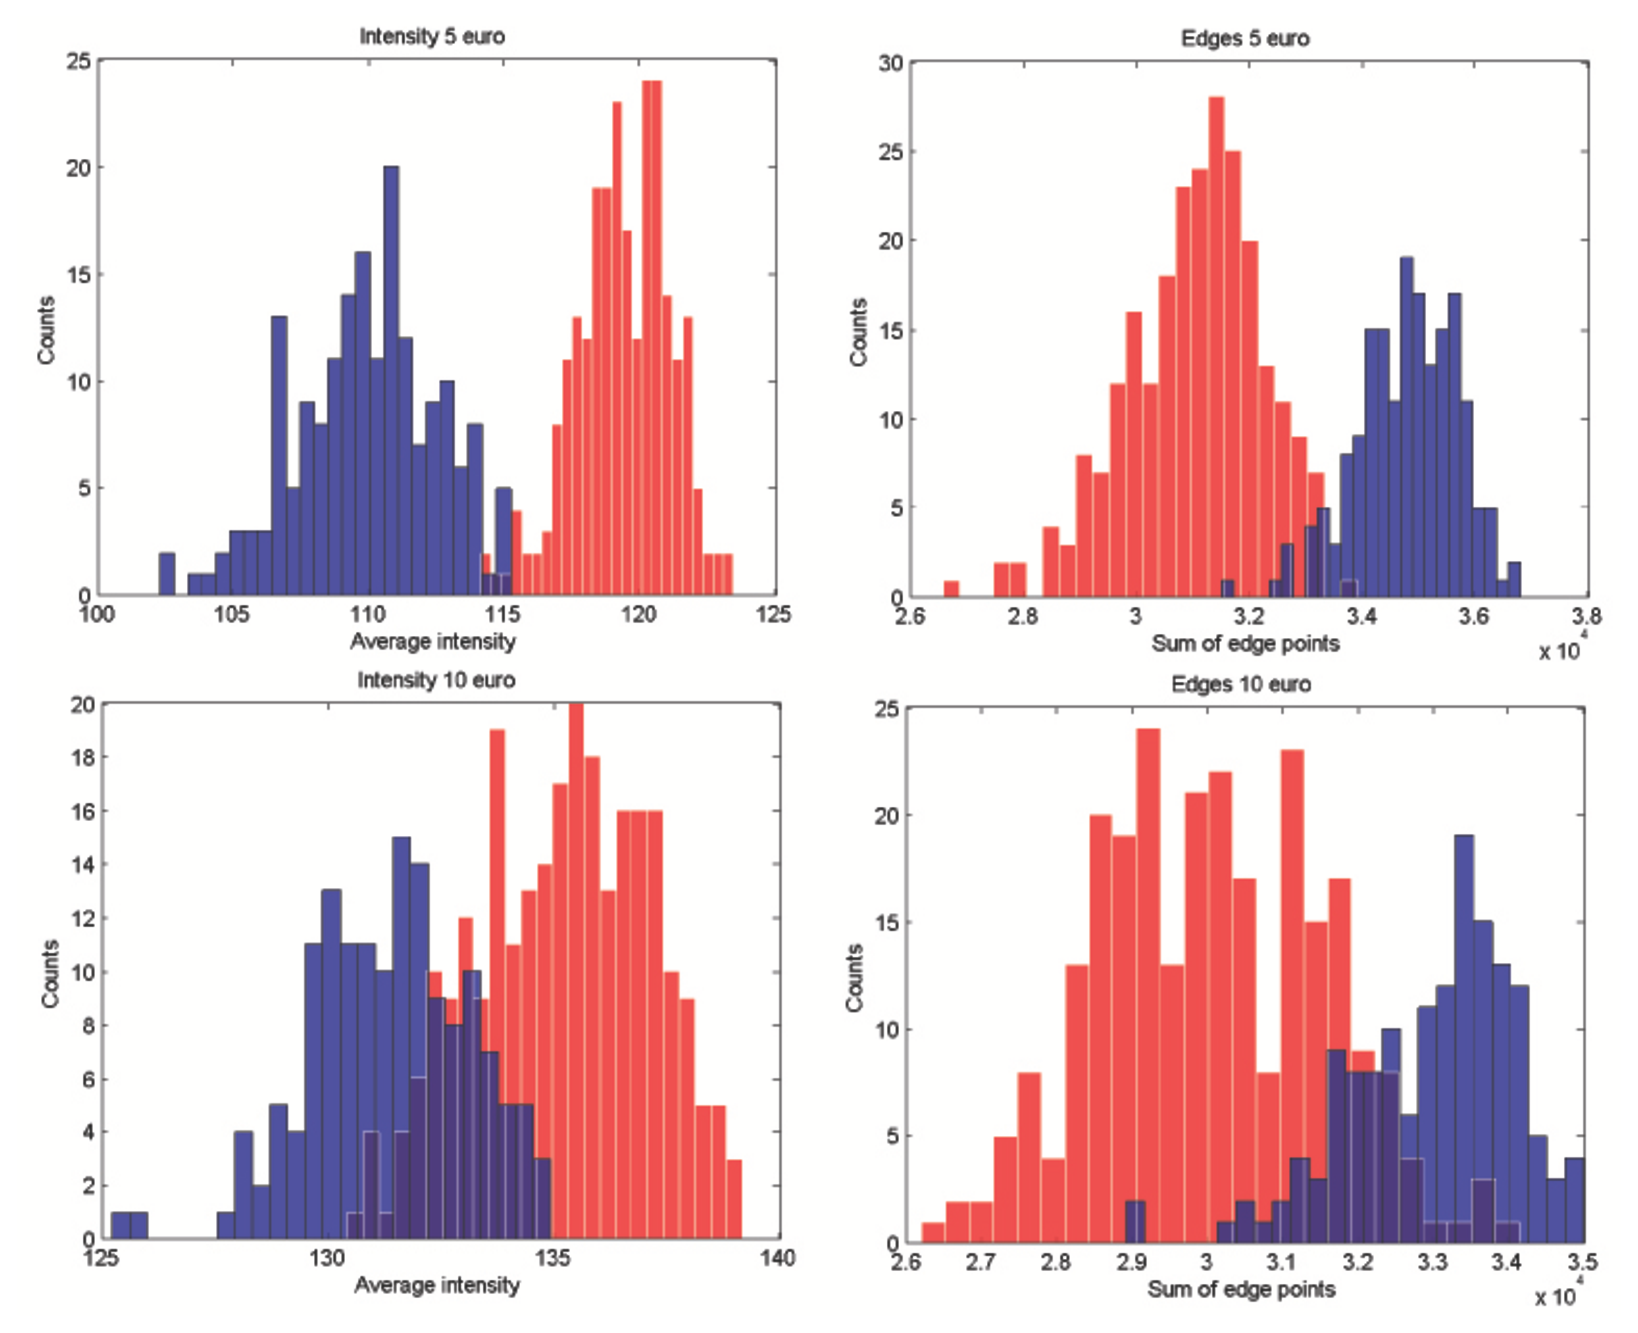
\epsfig{file=img/ie_histograms.eps, width=1\linewidth}
				\caption{plot of average intensity and edge count for 5 Euro bills}
				\label{histograms}
			\end{figure}


The idea of using the intensity is based on	the current approach used in the DNB (e.g. measuring the reflection of light on a small patch near the water mark). The second idea of using the edges is based on the assumption that dirty and old bills have significantly more wrinkles and folds than relative new bills. In the first simple implementation the raw intensity values of the image of the bill are used. This is done by segmenting the bills into smal overlappingl regions (9 by 23 showed best results). Over these regions the average intensity is calculated. In this way it is possible to retrieve two Gaussian distributions of the intensity of all the regions over all the images, one for clean bills and one for dirty bills. This provides a tool to compare the probability of a region on a bill belonging to a clean or dirty bill. Here again we apply \emph{Naive Bayes} in order to make use of the prior knowledge available.
			
			In the edge approach the image is first filtered using the Canny-edge detector. The Canny edge filter works in 5 steps: 
			
			\begin{itemize} 
				\item Step 1: Gaussian smoothing 
				\item Step 2: Extract the gradient of the image by convolving the image with 2 kernels, one to find the derivative in the X direction and one to find the derivative in the Y direction				
				\item Step 3: Determine the direction of the edge using results from step 2  
				\item Step 4: Apply non-maximum suppression to find the real edge (selecting only the maximum edge points found)
				\item Step 5: Finally the hysterisis is used to make the lines continue
            \end{itemize} 
            
            The result of an image for a bill after applying Canny edge filter
            can be seen in Figure \ref{canny5Euro}.
            
            \begin{figure}[!hbtp]
				\centering 
				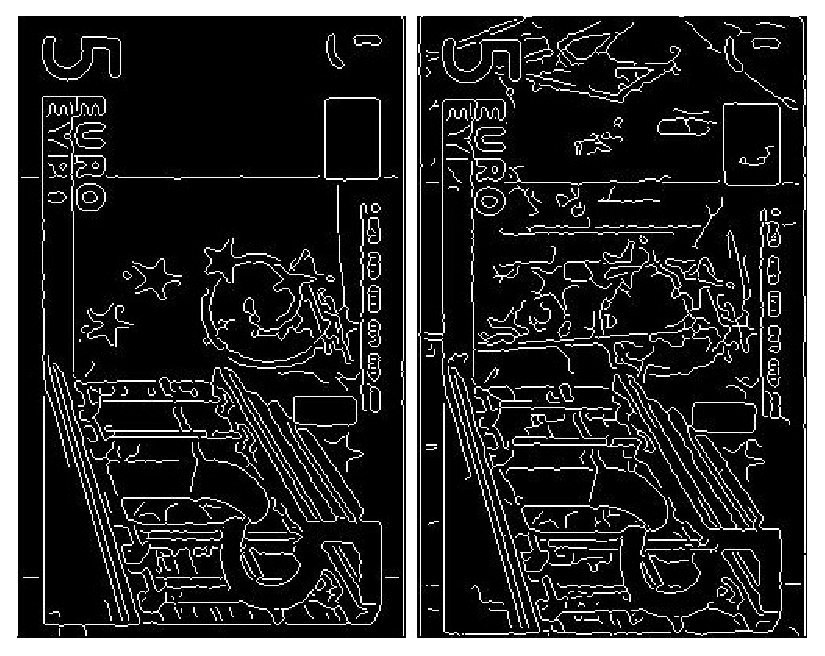
\epsfig{file=img/canny5euro.eps, width=1\linewidth}
				\caption{Results Canny edge filter. Left on a clean bill. Right on a dirty bill} 
				\label{canny5Euro} 
			\end{figure} 
			
			After applying the Canny edge filter to the images the resulting images are segmented in small regions. Per region the sum-of-edge-points is calculated. When doing this for all images we can again extract two Gaussian distributions of edge points per region (one for clean and one for dirty bills). Since calculating the average intensity and sum-of-edge-points only need to be calculated once, the learning phase is much faster compared to the other two techniques which makes it possible to have more convergence in finding the best model during training.
			
	\section{Results}\label{sec:results}
		The available image data set was split into a holdout-set and the remaining data was used to develop and train our algorithms on. The holdout-set consists of 60 fit and 40 unfit bills, selected randomly out of the total set of images (both for 5 and 10 Euro). During training, the remaining set was split up into a validation-set, a training-set and a test-set in order to perform \emph{random sub-sampling validation}.

		The whole process of defining the validation set and applying random sub-sampling validation was repeated several times to ensure a correct estimations of the error-rates. For each round of the validation, a model was trained using the \emph{AdaBoost algorithm} described in section \ref{sec:Methods}. The obtained model after training was tested by building the strong classifier and computing the corresponding confusion matrix values: \emph{true-positive estimation} (unfit classified as unfit), \emph{true-negative estimation} (fit classified as fit), \emph{false-positive estimation} (fit classified as unfit) and \emph{false-negative estimation} (unfit classified as fit).
		
		In order to derive a number of hypothesis to use for AdaBoost, we have plotted the error-rates for each technique with respect to a number of hypothesis. However, different decisions had to be made here for each technique since some take much longer to train.

		\subsection{Convolution Results}\label{sec:haar_results}
		%% 13x5 regions, overlapping 50% in total 1365 features
		Figure \ref{haar_plot10} and Figure \ref{haar_plot5} show how the error evolves depending on the number of models for the 10 Euro bills, respectively for the 5 Euro bills. Due to the fact that the number of features generated for only 21 patterns and a segmentation for each image of 9 (in the x-direction) by 23 (in the y-direction) overlapping regions gives a total of 4,347 features, the training part will be relatively slow for this method. In order to create reliable models we have used 5 repetitions, 10 hypothesis (features to be chosen by AdaBoost), 10 trials in the random sub-sampling validation method. The choice for 10 hypothesis is based on the fact that for 10 Euro bills the error-rate got stable around this number, and using more hypothesis would result in time consuming learning trials.

		In Figure \ref{haar_regions10} are indicated the most voted regions for the 10 Euro bills in \emph{AdaBoost} throughout all trials and all repetitions. We can notice that for the front of the bills the regions selected are mainly positioned on the water mark area, while for the rear side of the bills, there are some regions considered as being the most informative on the white patch, but also the area in the middle is selected as containing discriminative information. This could be explained by the fold in the middle of the bills.

		\begin{figure}[!hbtp]
			\centering
			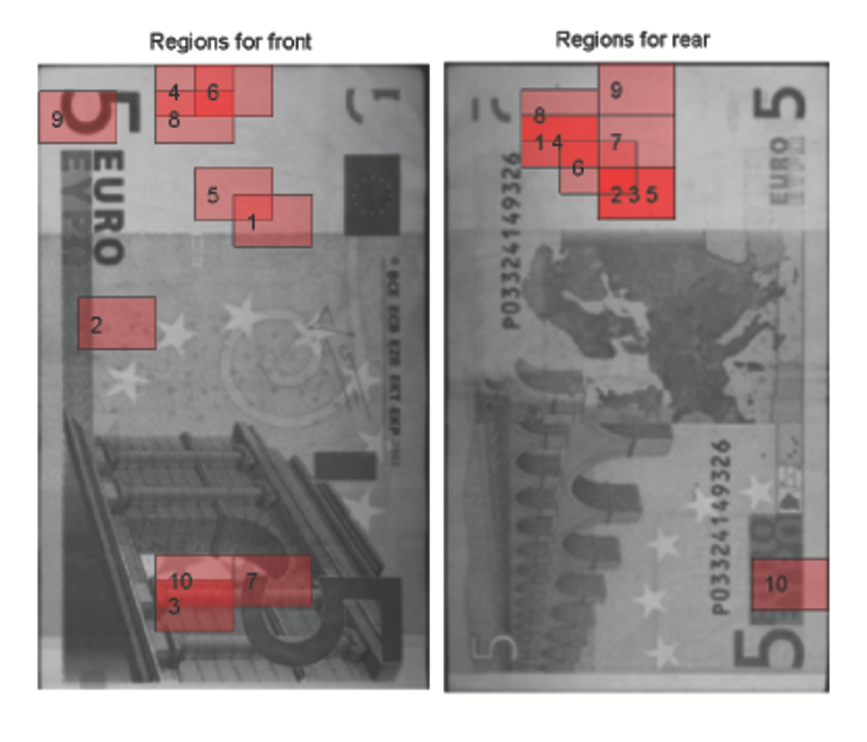
\epsfig{file=img/5x12_haar_regions5.eps, width=1\linewidth}
			\caption{Best regions for 5 Euro bills (Haar)}
			\label{haar_regions5}
		\end{figure}

		Figure \ref{haar_regions5} shows the most voted regions for the 5 Euro bills in \emph{AdaBoost} throughout all trials and all repetitions. For the 5 Euro bills the regions for front and rear that were chosen as being the most informative ones are again mainly around the water mark area, but unlike those for 10 Euro bills, the regions for front side are the ones that are more spread throughout the image.

		Figure \ref{haar_plot5} and Figure \ref{haar_plot10} indicate how the error evolves with respect to the number of hypothesis chosen to be used in the \emph{AdaBoost} technique. From the two images it can be noticed that the values obtained when using 10 features in the final model seems to perform better in general compared to a smaller number of features.

		\begin{figure}[!hbtp]
			\centering
			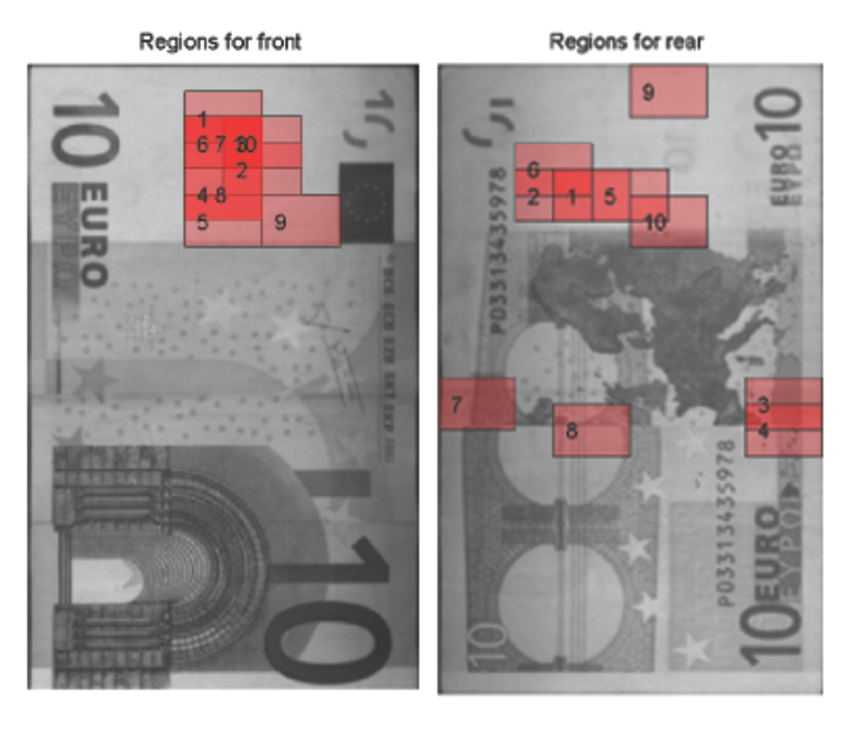
\epsfig{file=img/5x12_haar_regions10.eps, width=1\linewidth}
			\caption{Best regions for 10 Euro bills (Haar)}
			\label{haar_regions10}
		\end{figure}

		\begin{figure}[!hbtp]
			\centering
			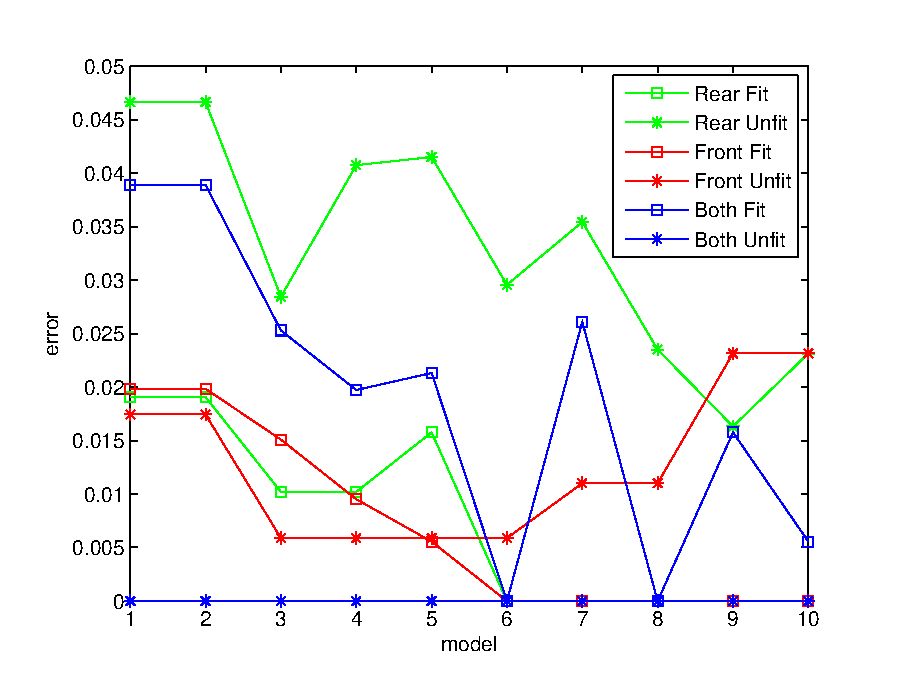
\epsfig{file=img/haar_plot5.eps, width=1\linewidth}
			\caption{Error depending on the number of features - 5 Euro bills (Haar)}
			\label{haar_plot5}
		\end{figure} 

		\begin{figure}[!hbtp]
			\centering
			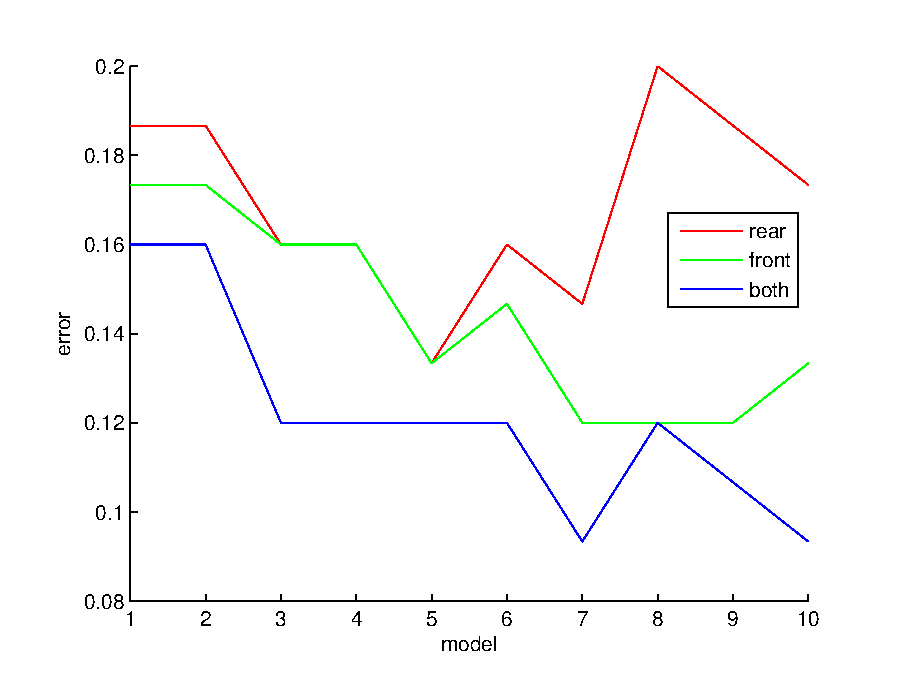
\epsfig{file=img/haar_plot10.eps, width=1\linewidth}
			\caption{Error depending on the number of features - 10 Euro bills (Haar)}
			\label{haar_plot10}
		\end{figure} 

		\subsection{PCA Results}\label{sec:pca_results}
			Defining the number of regions to perform PCA on was derived from a few experiments on different number of segments. When trying too small segments, the information captured by PCA could not represent the dirt on the bills anymore. When defining the segments too large, the information gets too general, and similar results are measured as for the whole bill. Dividing the bill into 3 (in the x-direction) by 7 (in the y-direction) regions gave promising error-rates during the training part as can be seen in Figure \ref{pca_plot5} and Figure \ref{pca_plot10}. Surprisingly, the number of regions that need to be chosen to get a maximal error of 5\% on unfit bills (the baseline for DNB) is only measured at 1 and 2 weak classifiers. Because the error for the fit bills is lowest when using one weak classifier only, the final model is trained on finding only one region. The most discriminating regions can be seen in Figure \ref{pca_regions5} and Figure \ref{pca_regions10}. Note that the learning process of this technique is very slow because after obtaining a new train- and test-set during random sub-sampling validation the eigen-faces for every region need to be calculated.

		\begin{figure}[!hbtp]
			\centering
			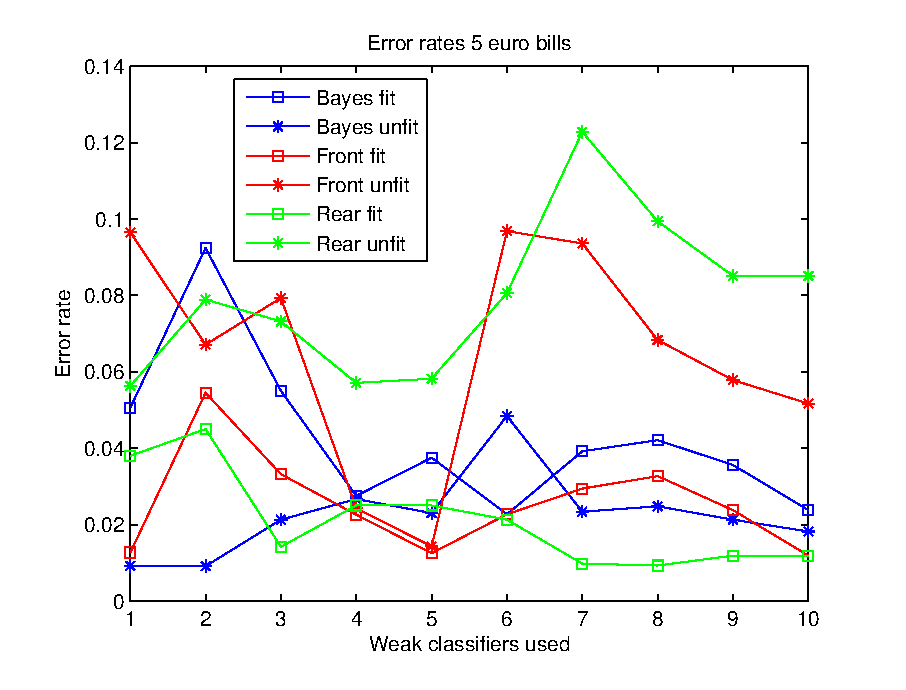
\epsfig{file=img/pca_plot5.eps, width=1\linewidth}
			\caption{Error depending on the number of features - 5 Euro bills (PCA)}
			\label{pca_plot5}
		\end{figure}

		\begin{figure}[!hbtp]
			\centering
			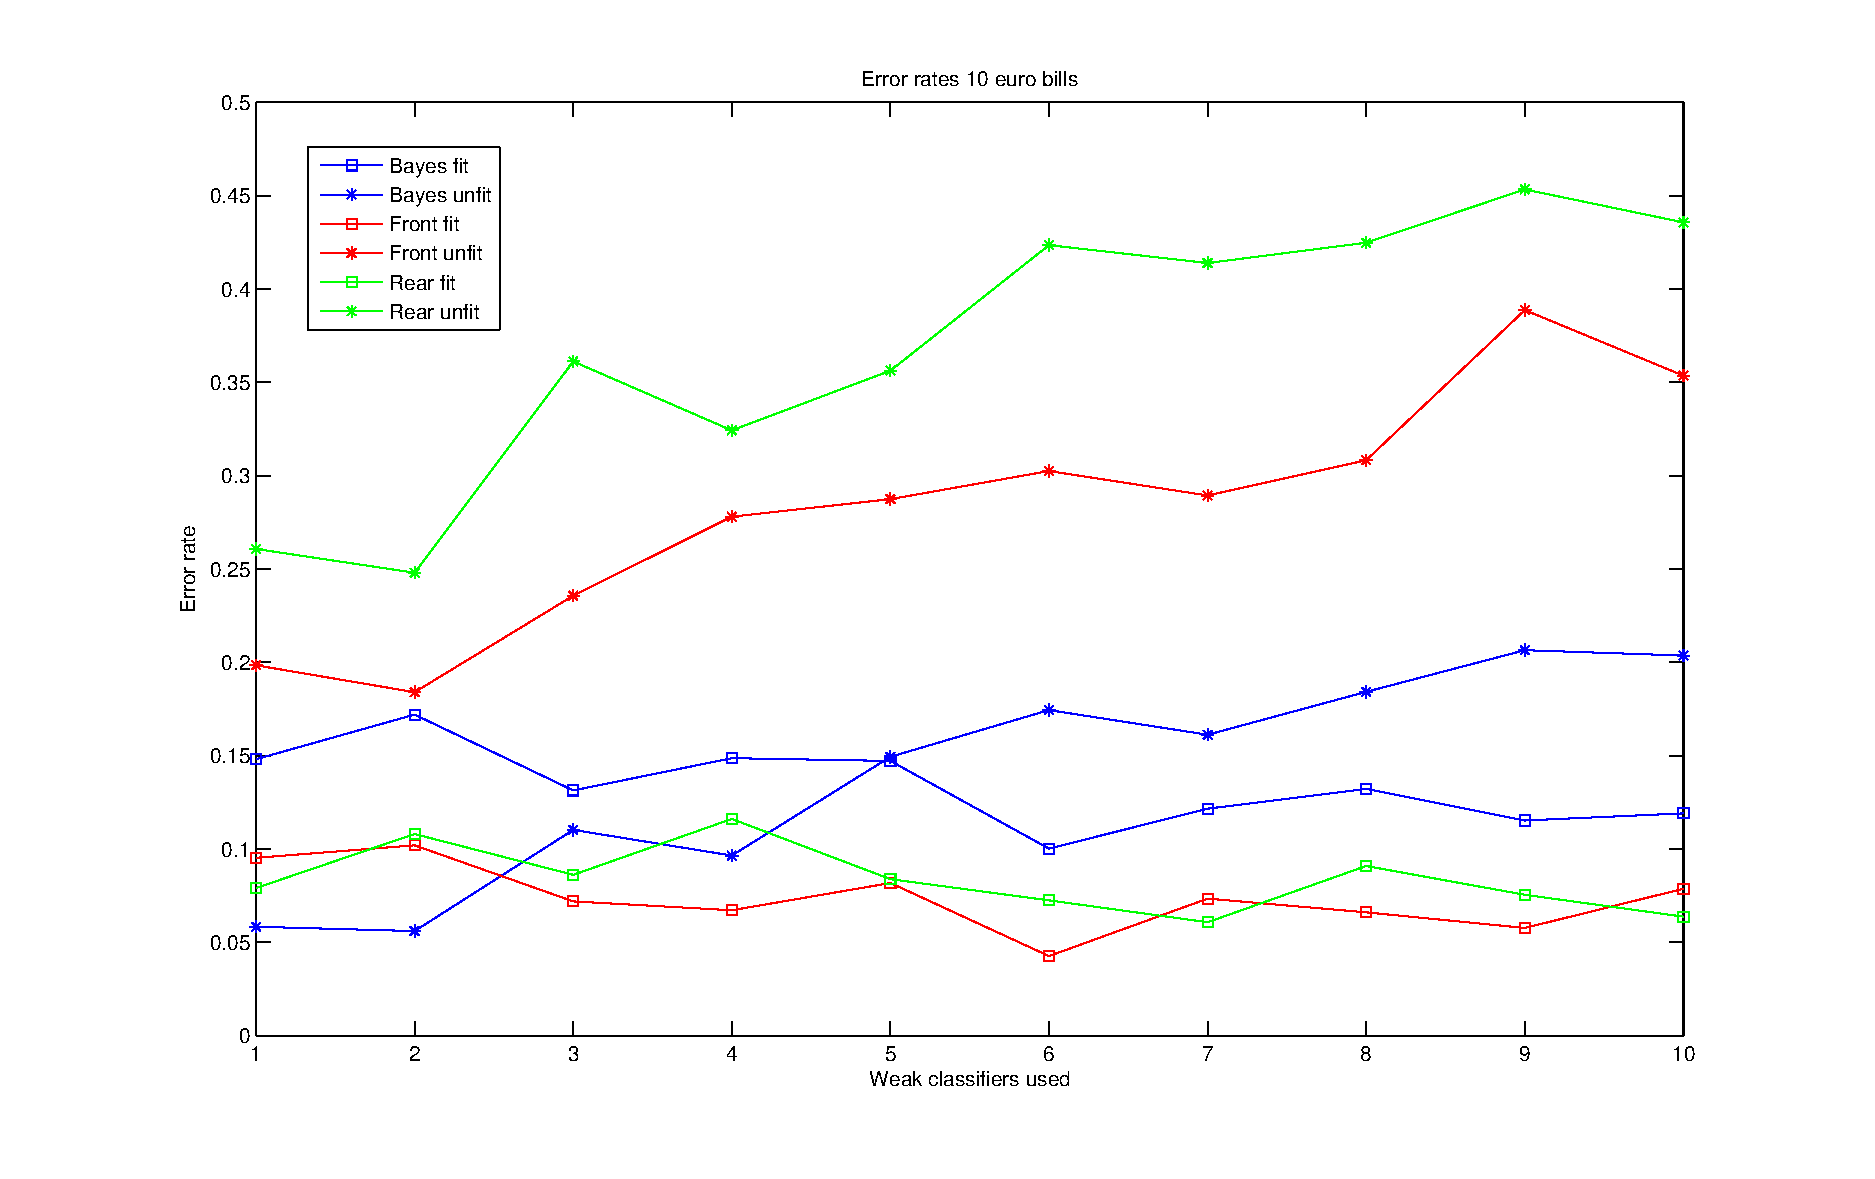
\epsfig{file=img/pca_plot10.eps, width=1\linewidth}
			\caption{Error depending on the number of features - 10 Euro bills (PCA)}
			\label{pca_plot10}
		\end{figure}

		\begin{figure}[!hbtp]
			\centering
			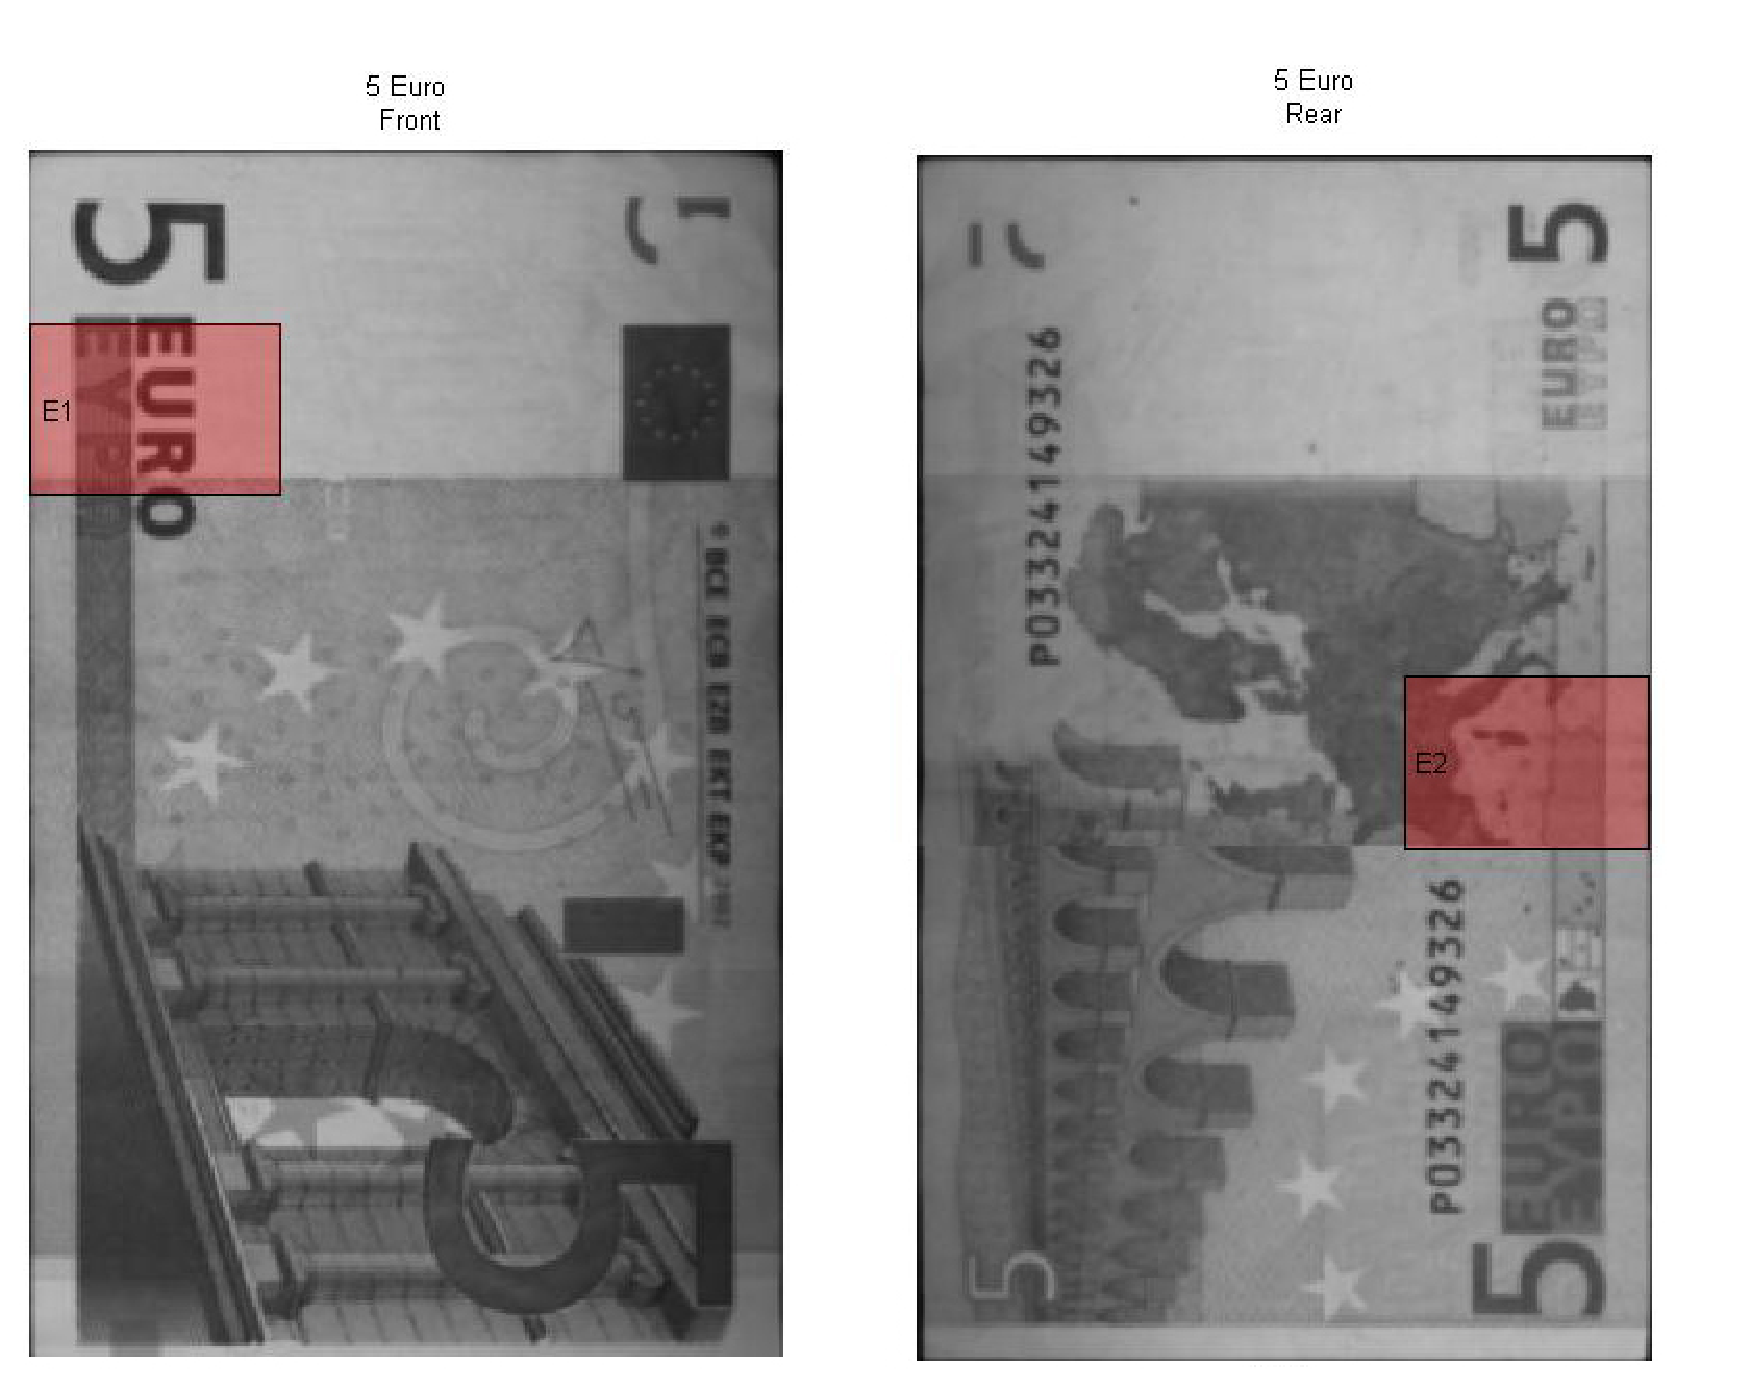
\epsfig{file=img/pca_regions5.eps, width=1\linewidth}
			\caption{Best regions for 5 Euro bills (PCA)}
			\label{pca_regions5}
		\end{figure}
		\begin{figure}[!hbtp]
			\centering
			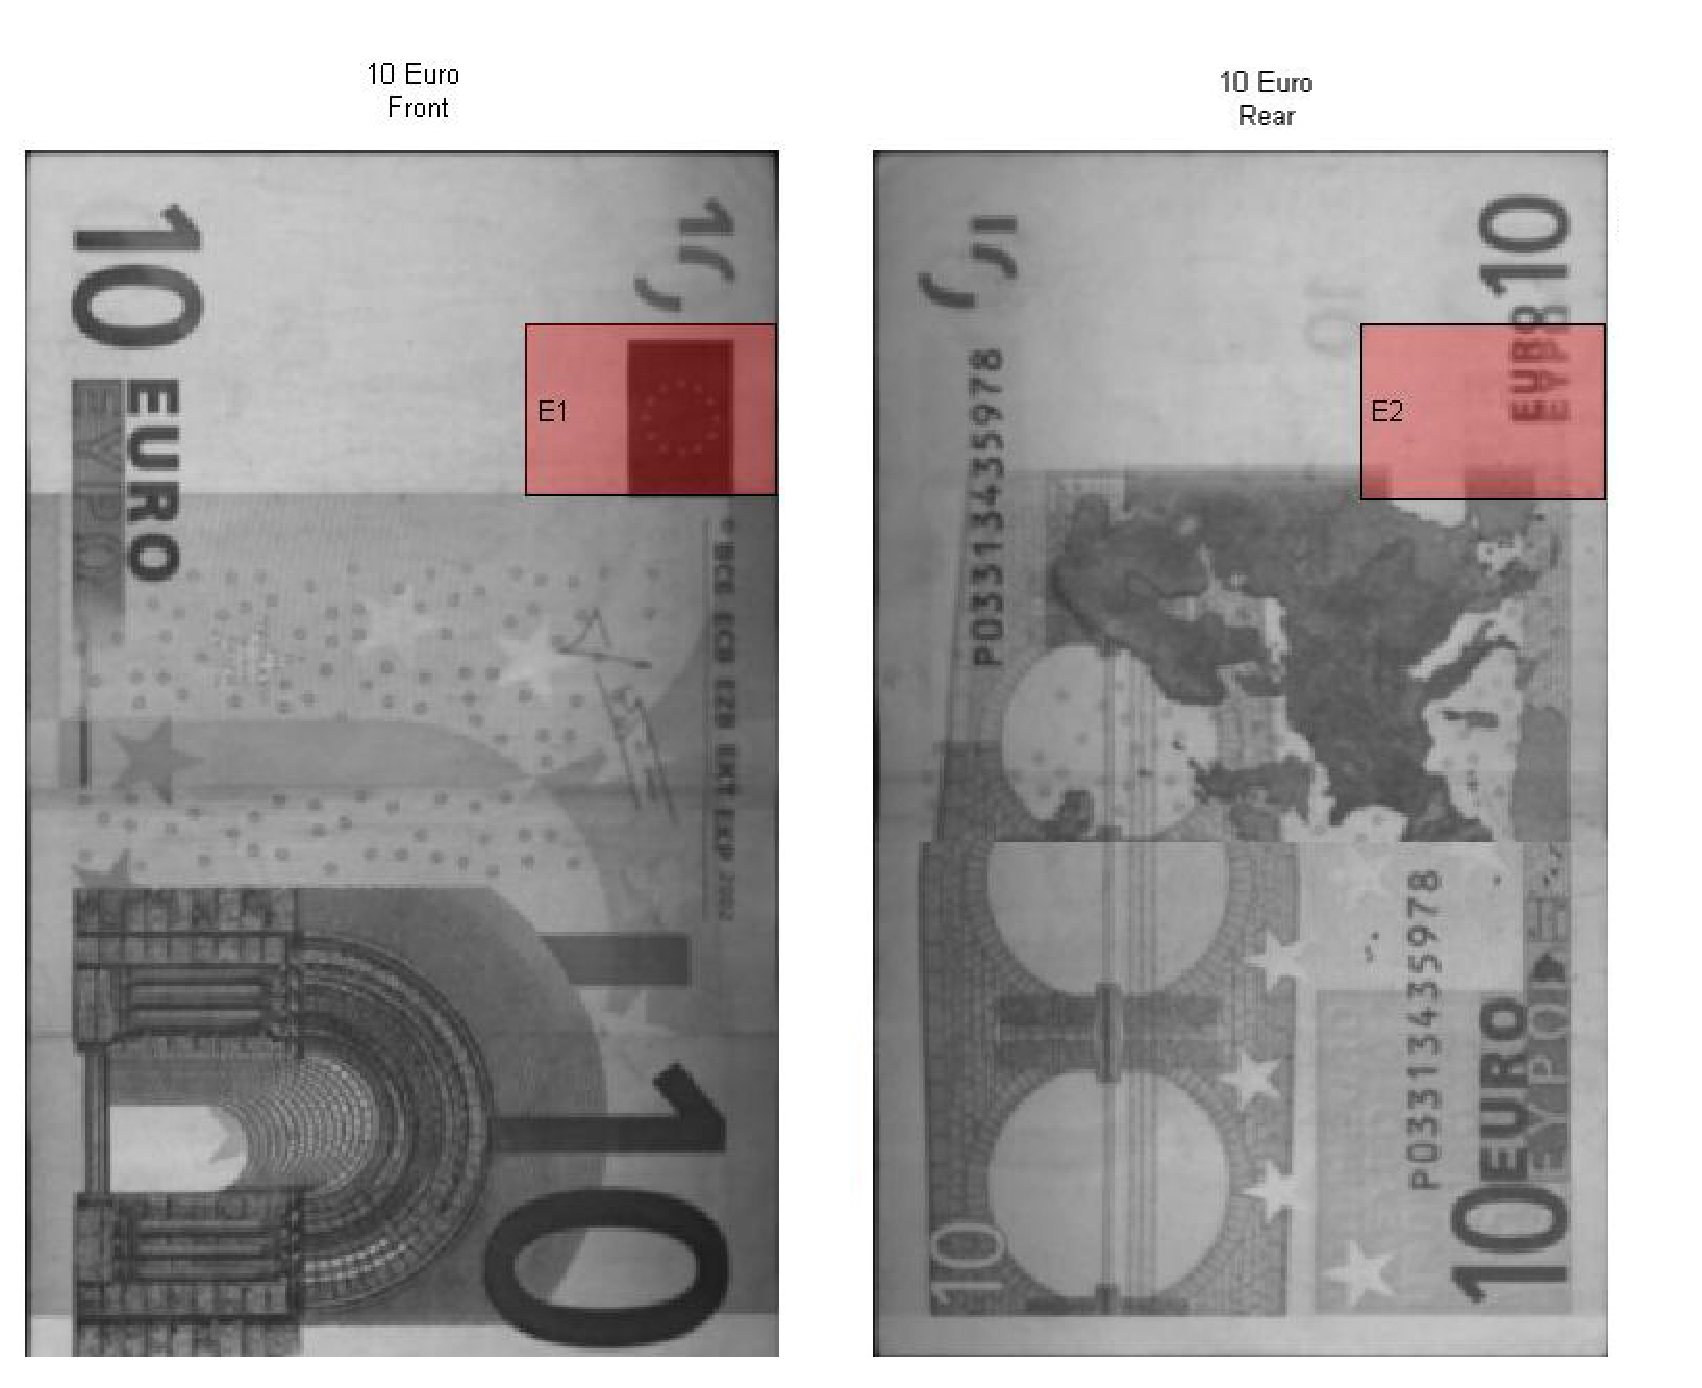
\epsfig{file=img/pca_regions10.eps, width=1\linewidth}
			\caption{Best regions for 10 Euro bills (PCA)}
			\label{pca_regions10}
		\end{figure}
		
		
		\subsection{Intensity \& Edges Results}\label{sec:ie_results}
			For the intensity and edges implementation we also used overlapping regions, 9 (in the x-direction) by 23 (in the y-direction) for front and for the rear of the bill. This results in 414 features. For every region there is only one value that represents the edge count or the average intensity, thus there is a relative small amount of models to train on. Therefore we could run bigger tests in order to achieve reliable models. In order to create these models we have used 40 repetitions, 40 hypotheses and 40 random sub-sampling validation runs. To determine the optimal number of weak classifiers to use for the 5 and 10 Euro bills we have plotted the errors with respect to the number of weak classifiers used. We choose the weak classifiers that reduced the error "substantially" (see Figure \ref{IE_plot5} and Figure \ref{IE_plot10} for the 10 Euro and 5 Euro plots). For the 10 Euro bills we used 40 weak classifiers and for the 5 Euro we used 10 classifiers. Figure \ref{ie_regions5} and Figure \ref{ie_regions10} indicate the selected areas on 10 and 5 Euro bills. The blue rectangles represent the regions found as being the most representative ones for intensity, while the red regions indicate the most discriminative regions when using edge detection.

		\begin{figure}[!hbtp]
			\centering
			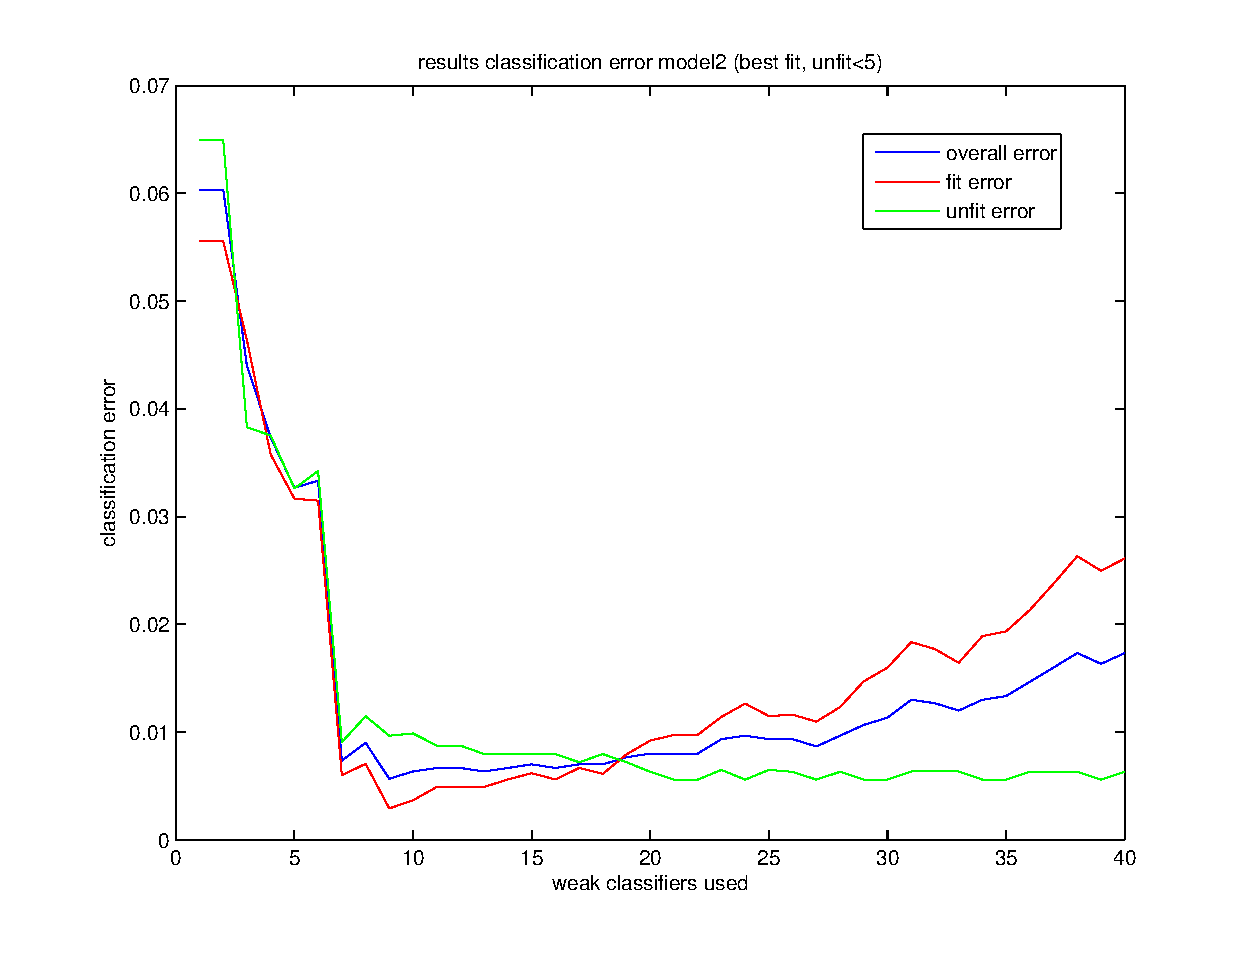
\epsfig{file=img/IE5eurPlot.eps, width=1\linewidth}
			\caption{Error depending on the number of features - 5 Euro bills (IE)}
			\label{IE_plot5}
		\end{figure} 

		\begin{figure}[!hbtp]
			\centering
			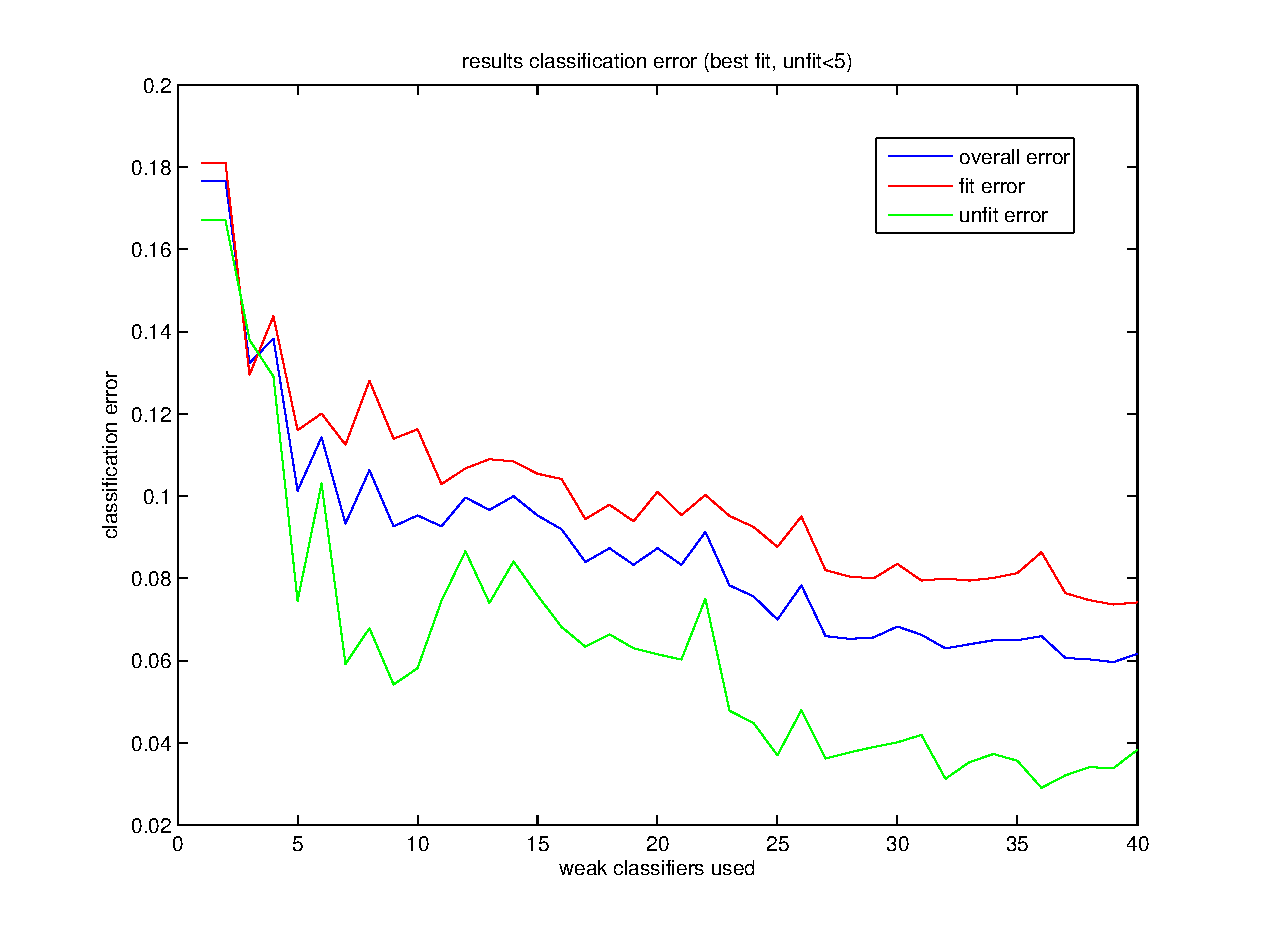
\epsfig{file=img/IE10eurPlot.eps, width=1\linewidth}
			\caption{Error depending on the number of features - 10 Euro bills (IE)}
			\label{IE_plot10}
		\end{figure} 
		
		\begin{figure}[!hbtp]
			\centering
			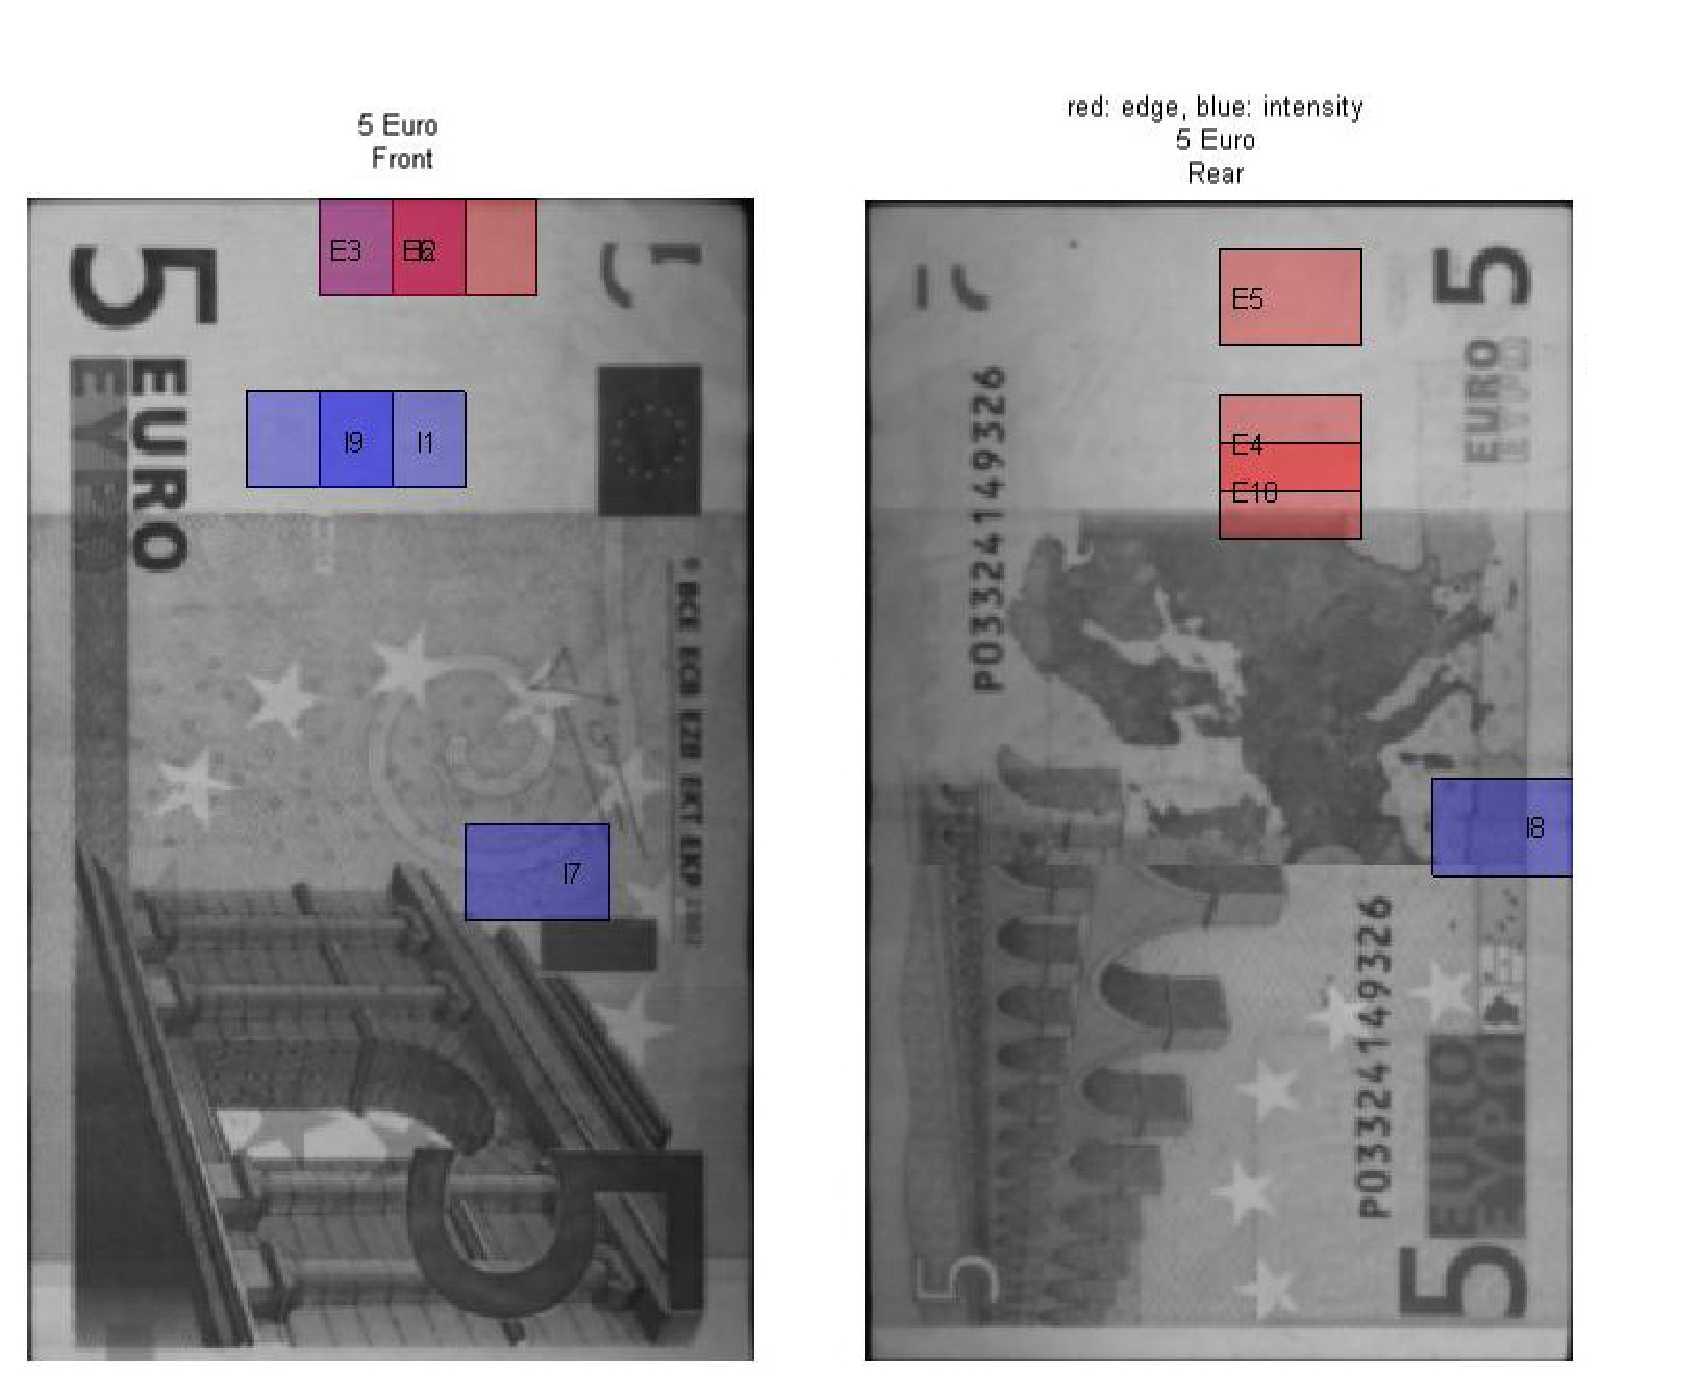
\epsfig{file=img/5x12_ie_regions5.eps, width=1\linewidth}
			\caption{Best regions for 5 Euro bills (IE)}
			\label{ie_regions5}
		\end{figure}
		
		\begin{figure}[!hbtp]
			\centering
			\epsfig{file=img/5x12_ie_regions10b.eps, width=1\linewidth}
			\caption{Best regions for 10 Euro bills (IE)}
			\label{ie_regions10}
		\end{figure}
		
					
		\subsection{Combined Results}\label{sec:comb_results}
			Once all the strong classifiers for each of the methods above have been generated, we have combined their predictions using \emph{Naive Bayes} rule. Since all of our final models are prepared with a number of hypothesis which are equal or below the 5\% baseline from DNB, we choose to bias the Naive Bayes towards the fit bills with the motivation that there are more fit bills being destroyed relative to the number of unfit bills. The combined classifiers are tested on our holdout-set of 100 bills for each 5 and 10 Euro.

			The results for 10 Euro bills, respectively 5 Euro bills are shown in the Table \ref{table10} and Table \ref{table5}. For the 5 Euro bills the performance of both single classifiers Haar and IE look very promising already, and in combination we can only expect them to be as good or slightly worse in performance.

			\begin{table}[!htbp]
				\caption{Results for 5 Euro bills}
				\fontfamily{ccr}\selectfont\small
				\label{table5}
				\centering 
				\begin{tabular}{ | c | c | c|}
					\hline\hline & \emph{Fit Error} & \emph{Unfit Error} \\ [0.5ex]\hline 
					\emph{Haar} & 0 & 0 \\ [0.5ex]\hline
					\emph{IE} & 0.033 & 0 \\ [0.5ex]\hline
					\emph{PCA} & 0.083 & 0.025 \\ [0.5ex]\hline
					\emph{Haar \& IE} & 0 & 0 \\ [0.5ex]\hline
					\emph{Haar \& PCA} & 0 & 0.025 \\ [0.5ex]\hline
					\emph{IE \& PCA} & 0.033 & 0.025 \\ [0.5ex]\hline
					\emph{Haar \& IE \& PCA} & 0.033 & 0 \\ [0.5ex]\hline
				\end{tabular}
				\label{table:nonlin5eur} 
			\end{table}

			\begin{table}[!htbp]
				\caption{Results for 10 Euro bills}
				\fontfamily{ccr}\selectfont\small
				\label{table10}
				\centering 
				\begin{tabular}{ | c | c | c|}
					\hline\hline & \emph{Fit Error} & \emph{Unfit Error} \\ [0.5ex]\hline 
					\emph{Haar} & 0.05 & 0.15 \\ [0.5ex]\hline
					\emph{IE} & 0.033 & 0.13 \\ [0.5ex]\hline
					\emph{PCA} & 0.083 & 0.05 \\ [0.5ex]\hline
					\emph{Haar \& IE} & 0.017 & 0.23 \\ [0.5ex]\hline
					\emph{Haar \& PCA} & 0.017 & 0.2 \\ [0.5ex]\hline
					\emph{IE \& PCA} & 0.017 & 0.17 \\ [0.5ex]\hline
					\emph{Haar \& IE \& PCA} & 0.017 & 0.05 \\ [0.5ex]\hline
				\end{tabular} 
				\label{table:nonlin10eur} 
			\end{table}		
			

	\section{Conclusion}\label{sec:conclusion}
		From our experiments we have been able to learn the regions that contain the largest amount of information and help us distinguish between fit and unfit bills. These regions differ from one method to another, but in general the areas around the water-mark region and the middle of the bills have been proven to be the ones containing the most discriminative features.
		
		As it can be noticed from the results in section \ref{sec:comb_results}, combining different techniques can lead to an improvement in the performance of the final classifier although running single classifiers only gives great results as well. In terms of robustness it make sense to do combinations of strong classifiers for 5 and 10 Euro both bills, since the different techniques can cover different aspects of dirt on the bills. To test this hypothesis however, it is mandatory to have many more holdout-sets to test the final models on since our project does not give any proof on scalability yet.

		Although the results obtained using the various techniques discussed are very promising already, future work is possible and it should be mainly focused on finding a more powerful way of combining all the features used by all 3 techniques (Haar, PCA, Intensity \& Edge) into a strong classifier as AdaBoost can be capable of doing this. Also, combining the models for both front and rear can also be improved if certain prior knowledge can be incorporated.
		
		We would also recommend that special attention should be payed to the validity of certain features of the images from the data set by retrieving the origin on how the data-set is built up. We mention this because the results for average intensity are really promising, but this could be caused by bills being scanned in each class at a time and having differences in the intensity of the light possibly induced by the scanner being heated up.
	
		\bibliographystyle{alpha} 
		\begin{thebibliography}{3} 
			\bibitem{Haar}
				P. Viola \& M. Jones:\\
				\tit{Rapid Object Detection using a Boosted Cascade of Simple Features}
				(CVPR 2001)
			\bibitem{Ada}
				AdaBoost: \\
				\tit{http://en.wikipedia.org/wiki/AdaBoost}	
			\bibitem{MoNuSt}G. Molenaar, A. Nusselder and K. M. Stefanov: \\
				\tit{Classifying Bank Notes for Scheduled Destruction} (2009)
			\bibitem{Geusebroek} J.M. Geusebroek: \\
				\tit{Computer Vision for Banknote Sorting} (2009)		
		\end{thebibliography}		
\end{document}
